

\par Este trabalho está sendo desenvolvido mediante pesquisa explicativa a fim de entender como diferentes fatores modificam e afetam o desempenho das turbinas eólicas, buscando analisar e validar modelos teóricos. A figura \ref{fig:fluxogramaTCC} apresenta o fluxograma que ilustra o fluxo dessas etapas.  Desse modo, será adotado uma abordagem composta por procedimentos de pesquisa bibliográfica e documental, simulação computacional e análise de dados. 
\par Inicialmente, serão realizado estudos sobre perfis de vento, abordando as características atmosféricas e locais, determinando assim o potencial eólico, a curva de potência e a serie temporal. Em seguida, será desenvolvido o estudo e a modelagem dos componentes pertencentes a turbina eólica a fim de criar o modelo da turbina. 
\par Serão consultados artigos científicos, livros, teses, dissertações e publicações técnicas, além de documentos técnicos, como especificações de turbinas eólicas e relatórios de desempenho de sistemas eólicos.
\par A pesquisa será conduzida com base no perfil de vento da cidade de Cachoeira do Sul-RS. Este cenário foi escolhido devido às suas características de vento favoráveis para a geração de energia eólica.
\par Para o desenvolvimento e execução das simulações será utilizado o software MATLAB/ Simulink. Os dados de vento de Cachoeira do Sul serão integrados aos modelos, a fim de criar um cenário de simulação, a Figura \ref{fig:ilustracaoDoCenário} sintetiza de maneira ilustrativa o cenário a ser simulado. Elaborado o cenário, inicia-se o refinamento através de análise, que inclui a avaliação de métricas de desempenho, como eficiência de conversão de energia e comportamento dinâmico dos componentes. A validação dos modelos simulados será realizada comparando os resultados das simulações com dados teóricos e com dados disponíveis na literatura. 




\par Assim, dentre os objetos da pesquisa tem-se o desenvolvimento de uma plataforma de simulação de turbina eólica, que permite a modelagem e análise dos diversos componentes de uma turbina eólica. A pesquisa se concentra na modelagem teórica do comportamento do vento e dos componentes, como as pás, o rotor, o gerador e os sistemas de controle. Além disso, os dados de vento de Cachoeira do Sul são utilizados como base para as simulações teóricas, permitindo uma avaliação de inserção de aerogeradores na UFSM campus universitário de Cachoeira do Sul.

\begin{figure}[H]
    \caption{Fluxograma de desenvolvimento do projeto.}      
    \label{fig:fluxogramaTCC}
    \centering
    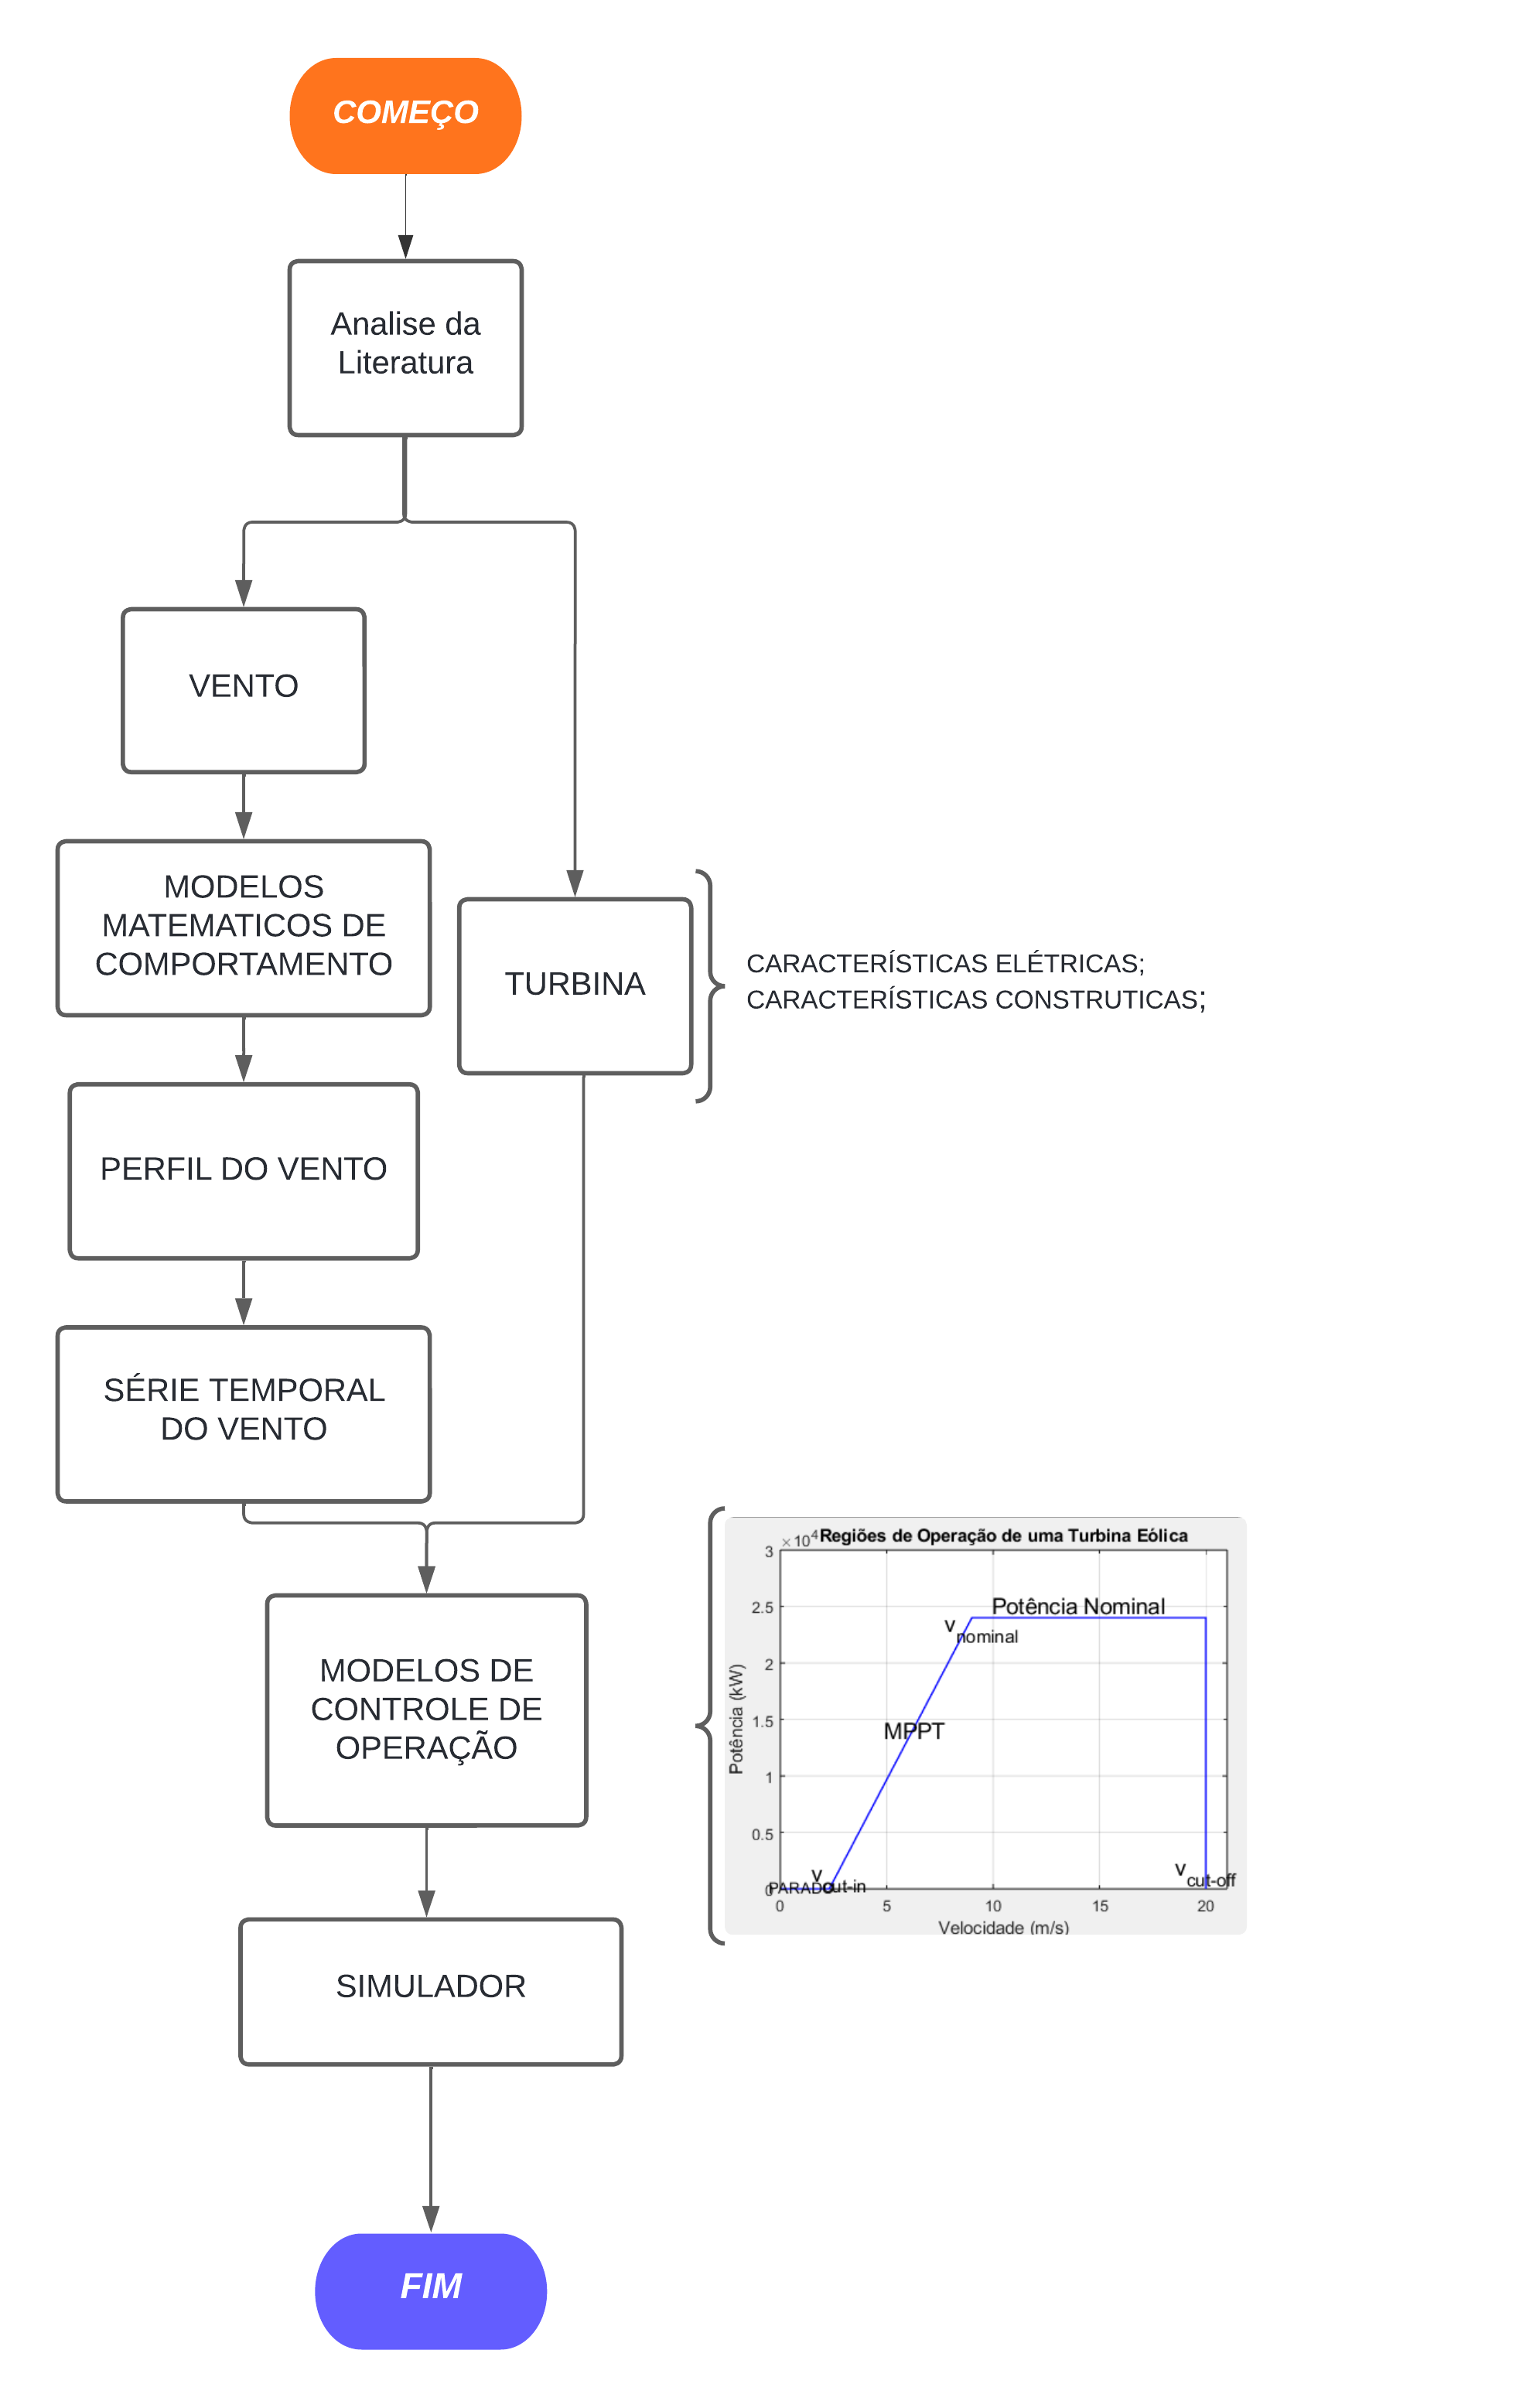
\includegraphics[width=0.8\textwidth]{Figuras/Teorico/TCC - AEROGERADOR.png}  
\end{figure}

\begin{figure}[H]
    \caption{Ilustração do cenário.}      
    \label{fig:ilustracaoDoCenário}
    \centering
    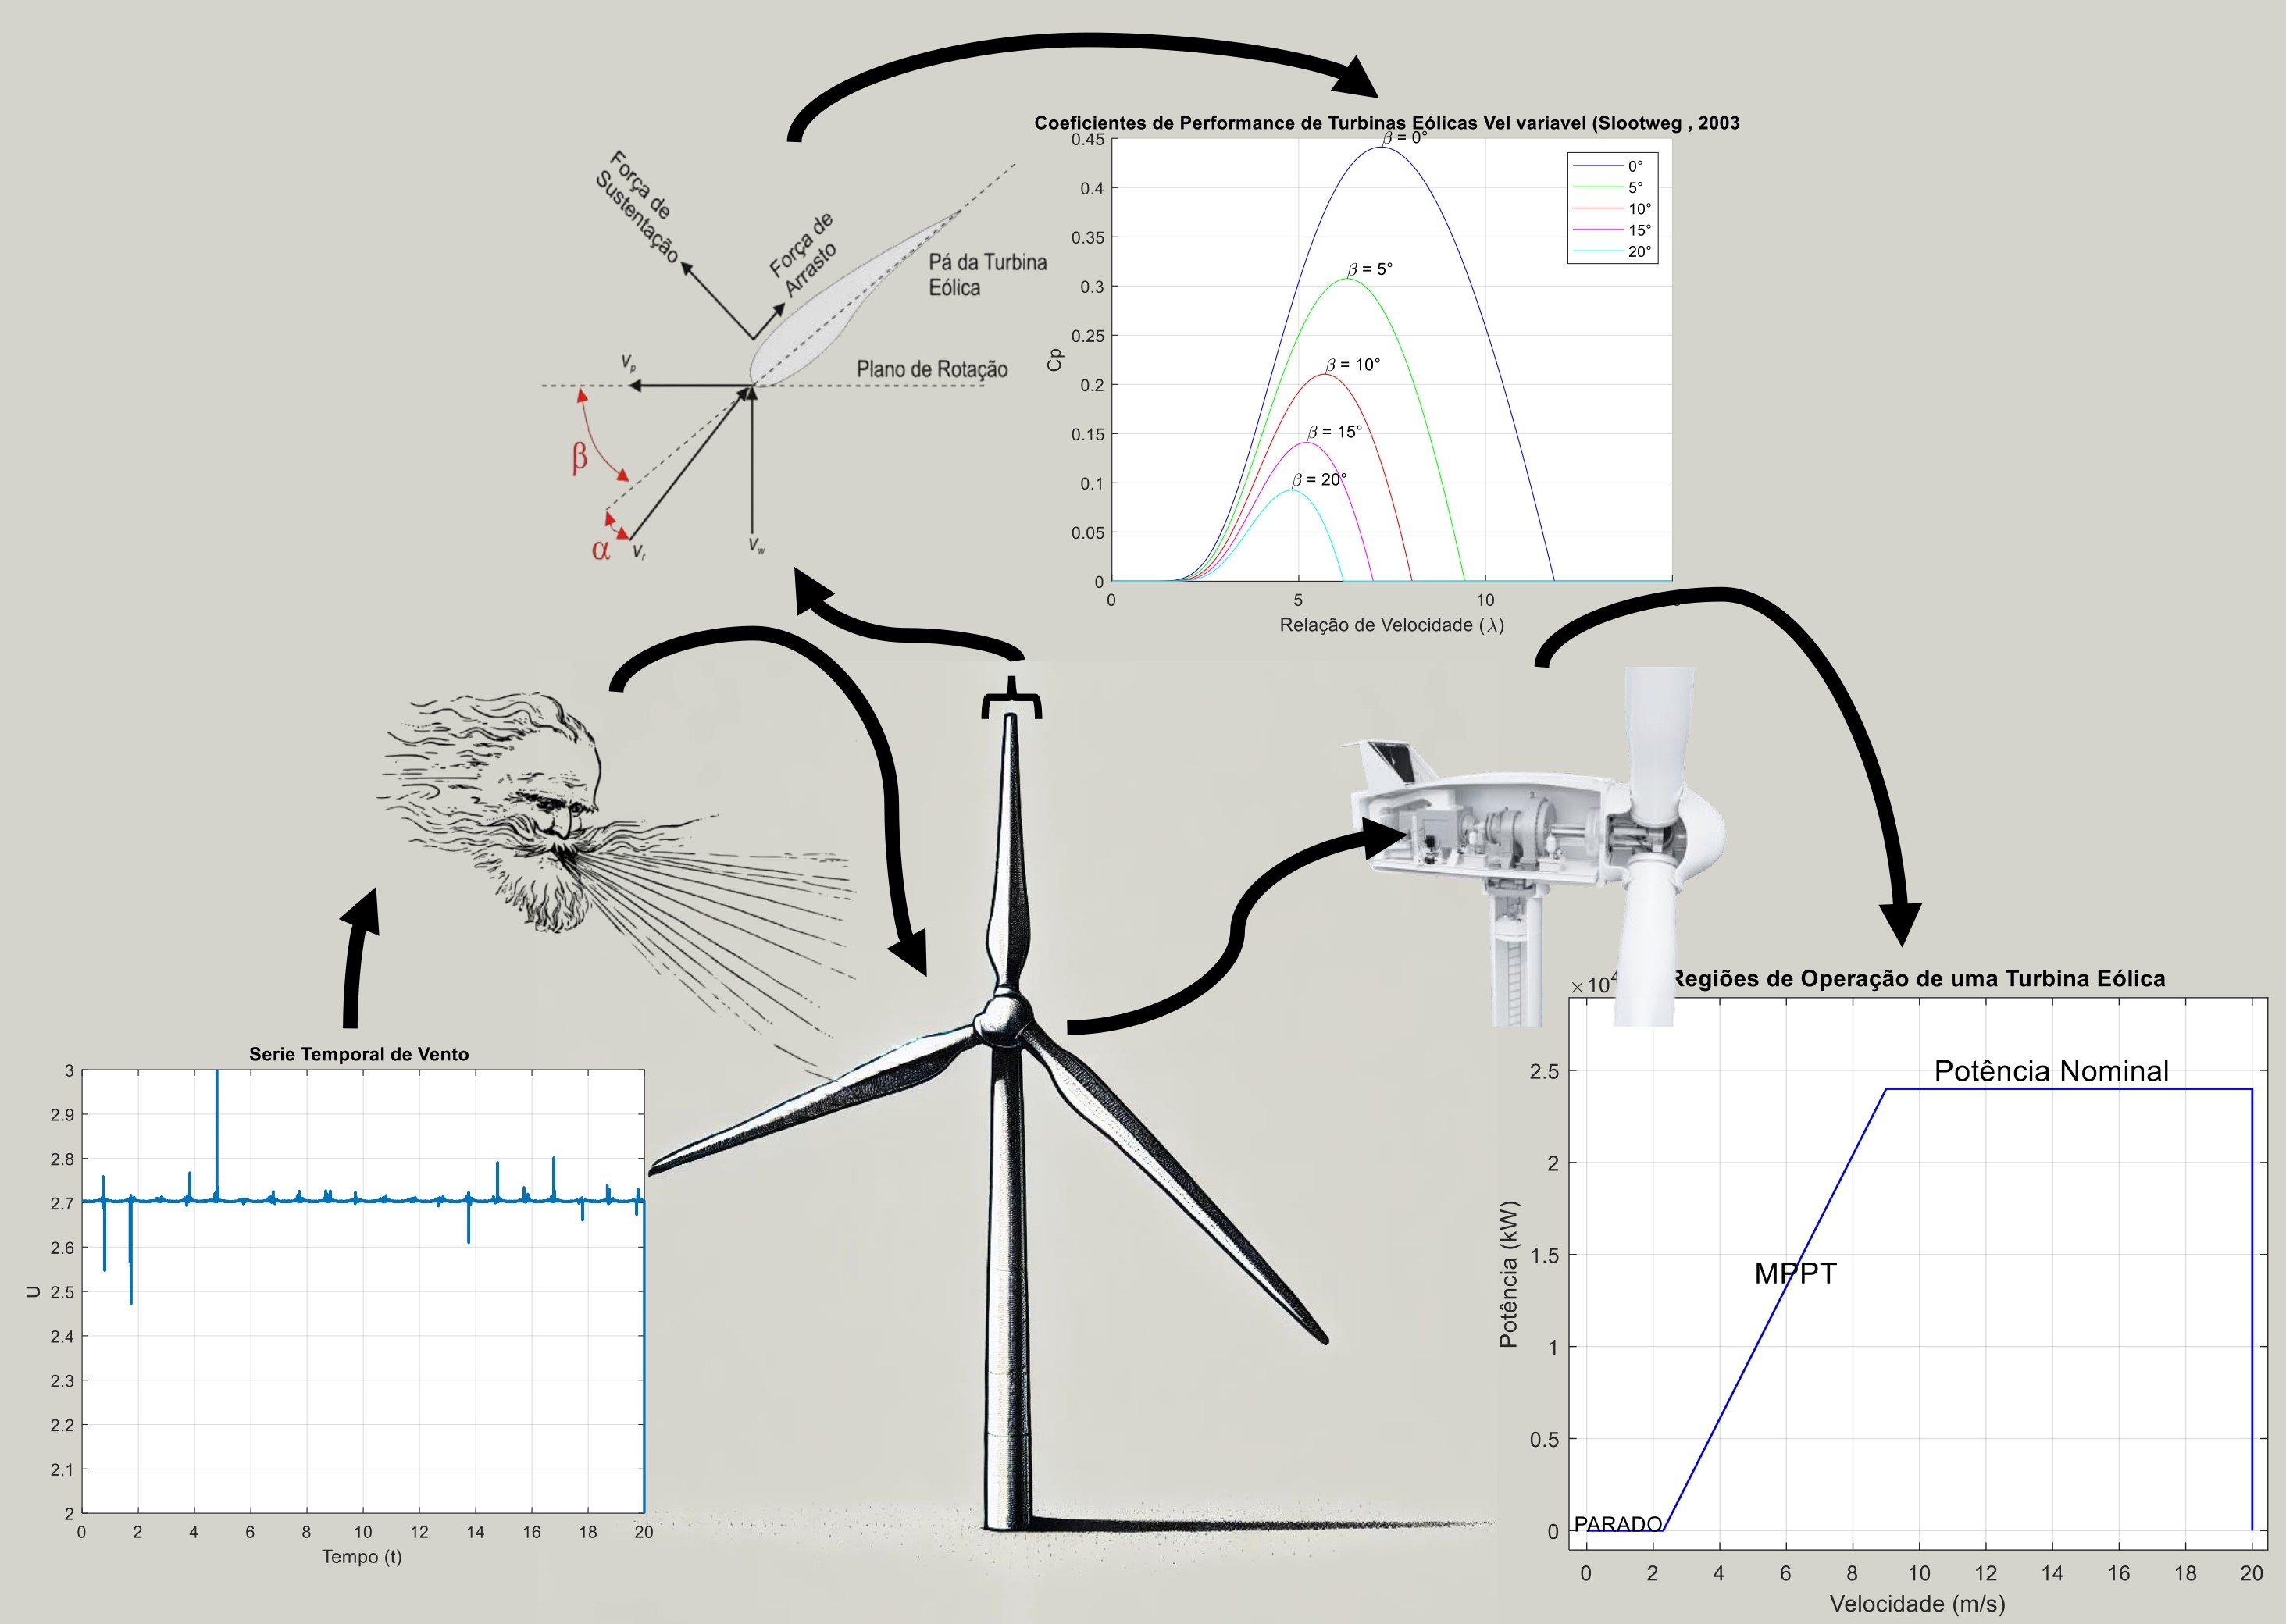
\includegraphics[width=0.8\textwidth]{Figuras/Teorico/metodologia_page-0001.jpg}  
\end{figure}
\section{Cronograma para Desenvolvimento do TCC II}
\par O cronograma a seguir detalha as atividades planejadas para o desenvolvimento da segunda parte do TCC, abordando os passos restantes para o desenvolvimento do trabalho. Este cronograma está organizado de agosto a dezembro. Cada ação está programada para ocorrer em períodos específicos, garantindo uma abordagem estruturada e organizada do projeto.
\begin{table}[h!]
\centering
\caption{Cronograma de ações}
\begin{tabular}{|m{5cm}|m{1cm}|m{1cm}|m{1cm}|m{1cm}|m{1cm}|m{1cm}|m{1cm}|m{1cm}|}
\hline
\textbf{Ação} &\textbf{AGO} & \textbf{SET} & \textbf{OUT} & \textbf{NOV} & \textbf{DEZ} \\ \hline
Analise para Modelos de Controle de Operação &  \cellcolor[gray]{0.8}& \cellcolor[gray]{0.8} & & & \\ \hline
Desenvolvimento do Sistema de Controle da Turbina & \cellcolor[gray]{0.8}  & \cellcolor[gray]{0.8} & \cellcolor[gray]{0.8} & & \\ \hline
Desenvolvimento da Plataforma de Simulação &  &  \cellcolor[gray]{0.8}&  \cellcolor[gray]{0.8}& & \\ \hline
Testes e Validação do Sistema &  &  & \cellcolor[gray]{0.8} & \cellcolor[gray]{0.8} & \\ \hline
Avaliação do Desempenho &  &  & \cellcolor[gray]{0.8} & \cellcolor[gray]{0.8} & \cellcolor[gray]{0.8} \\ \hline
Documentação e Preparação do Relatório Final &  &  &  &  \cellcolor[gray]{0.8}&  \cellcolor[gray]{0.8}\\ \hline
%Elaborar relatório final & & & & \cellcolor[gray]{0.8} & \cellcolor[gray]{0.8} \\ \hline
\end{tabular}
\end{table}
\par O cronograma é abordado em detalhes a seguir:
\begin{enumerate}
    \item \textbf{Análise para Modelos de Controle de Operação:} Será realizada a análise para o desenvolvimento dos modelos de controle de operação. Esta etapa é fundamental para entender as necessidades do sistema e definir os parâmetros de controle. 
    \item \textbf{Desenvolvimento do Sistema de Controle da Turbina:} Esta fase envolve a implementação de algoritmos de controle e ajustes necessários para otimizar o funcionamento da turbina.
    \item \textbf{Desenvolvimento da Plataforma de Simulação:} Início do desenvolvimento da plataforma de simulação. Esta etapa é crucial para integrar os modelos matemáticos e de controle em um ambiente de simulação.
    \item \textbf{Testes e Validação do Sistema:} Início dos testes e validação do sistema, verificando a precisão dos modelos e a eficácia dos controles implementados em estudos de casos envolvendo turbinas eólicas de velocidade variável.
    \item \textbf{Avaliação do Desempenho:} Início da avaliação do desempenho do sistema de simulação, analisando a eficácia e eficiência sob diferentes condições operacionais.
    \item \textbf{Documentação e Preparação do Relatório Final:} Compilação de toda a documentação do projeto e preparação do relatório final. Esta etapa inclui os resultados, conclusões e recomendações baseadas nas análises realizadas ao longo do projeto.
\end{enumerate}







%\chapter{Resultados}



